The field of particle physics saw the discovery of a variety of new particles in the 1950s and 60s.
At the time, their fundamental nature was unknown; however, due to their sheer number it seemed plausible that these particles, now known as mesons and baryons, were not elementary but composite.
Zweig~\cite{Zweig:1964jf} and Gell-Mann~\cite{GellMann:1964nj} independently proposed that mesons and baryons were in fact composed of spin-1/2 particles which Gell-Mann coined ``quarks''.
In this framework, mesons were bound states of a quark and an anti-quark while baryons were bound states of three quarks. More precisely, mesons and baryons are composed of their respective quarks, called valence quarks (which dictate the nucleon's quantum numbers), gluons (which mediate the strong force and bind the nucleon), and a sea of virtual quark-antiquark pairs~\cite{Yan:2015zoa}. 
The quark model of Zweig and Gell-Mann was initially met with some skepticism: it implied that quarks must have fractional charges of either 1/3 or 2/3 of the charge of the electron and that they violated the spin-statistics theorem.
The quantum number color~\cite{Greenberg:1964pe} was proposed to remedy the violation of the spin-statistics theorem and deep inelastic scattering experiments at SLAC~\cite{Breidenbach:1969kd,Bloom:1969kc} gave strong indications of the composite structure of the proton.

In attempting to describe the nature of inelastic electron-proton scattering, Bjorken proposed that the cross section for such a process was determined not by the absolute energy of the collision, but instead depended on dimensionless kinematic ratios~\cite{Bjorken:1969ja}.
This phenomenon, known as Bjorken scaling, was experimentally confirmed in experiments at SLAC~\cite{Prentki:1968fha}. 
Feynman interpreted Bjorken scaling in the following way~\cite{Feynman:1969ej}: hadrons behave as a collection of point-like constituents, or \emph{partons}, which each carry some fraction of the hadron's total energy.
Moreover, each of the partons can be described by a \emph{parton distribution function} (PDF), which gives the probability density for a parton to carry a given fraction of the hadron's total momentum.

The parton model assumes that quarks exist as free particles within the hadron, which is a good approximation for high energy electron-proton scattering in which the interactions between the electron and parton occur on a very short time scale through electromagnetic interactions mediated by photons.
This approximation breaks down for inelastic proton-proton scattering, in which the gluons which bind the proton together become relevant in the interaction and it is no longer valid to consider the partons as free particles.
In this regime, Bjorken scaling is no longer applicable, and the PDFs become dependent on the magnitude of the momentum transfer (frequently denoted by $Q^2$).
The PDF dependence on $Q^2$ cannot be calculated analytically; instead, the PDF can be measured through experiment at a particular value of $Q^2$ and then extrapolated to other values of $Q^2$ through the QCD evolution equations for parton densities~\cite{Altarelli:1977zs,Dokshitzer:1977sg,Gribov:1972ri}, also called the DGLAP equations.

The PDFs for the proton, as determined by the MSTW group~\cite{Martin:2009iq}, are shown in Fig.~\ref{fig:pp_nlo_pdfs} for $Q^2 = 10$ GeV and $Q^2 = 10^4$ GeV.
\begin{figure} [htbp!]
    \centering
    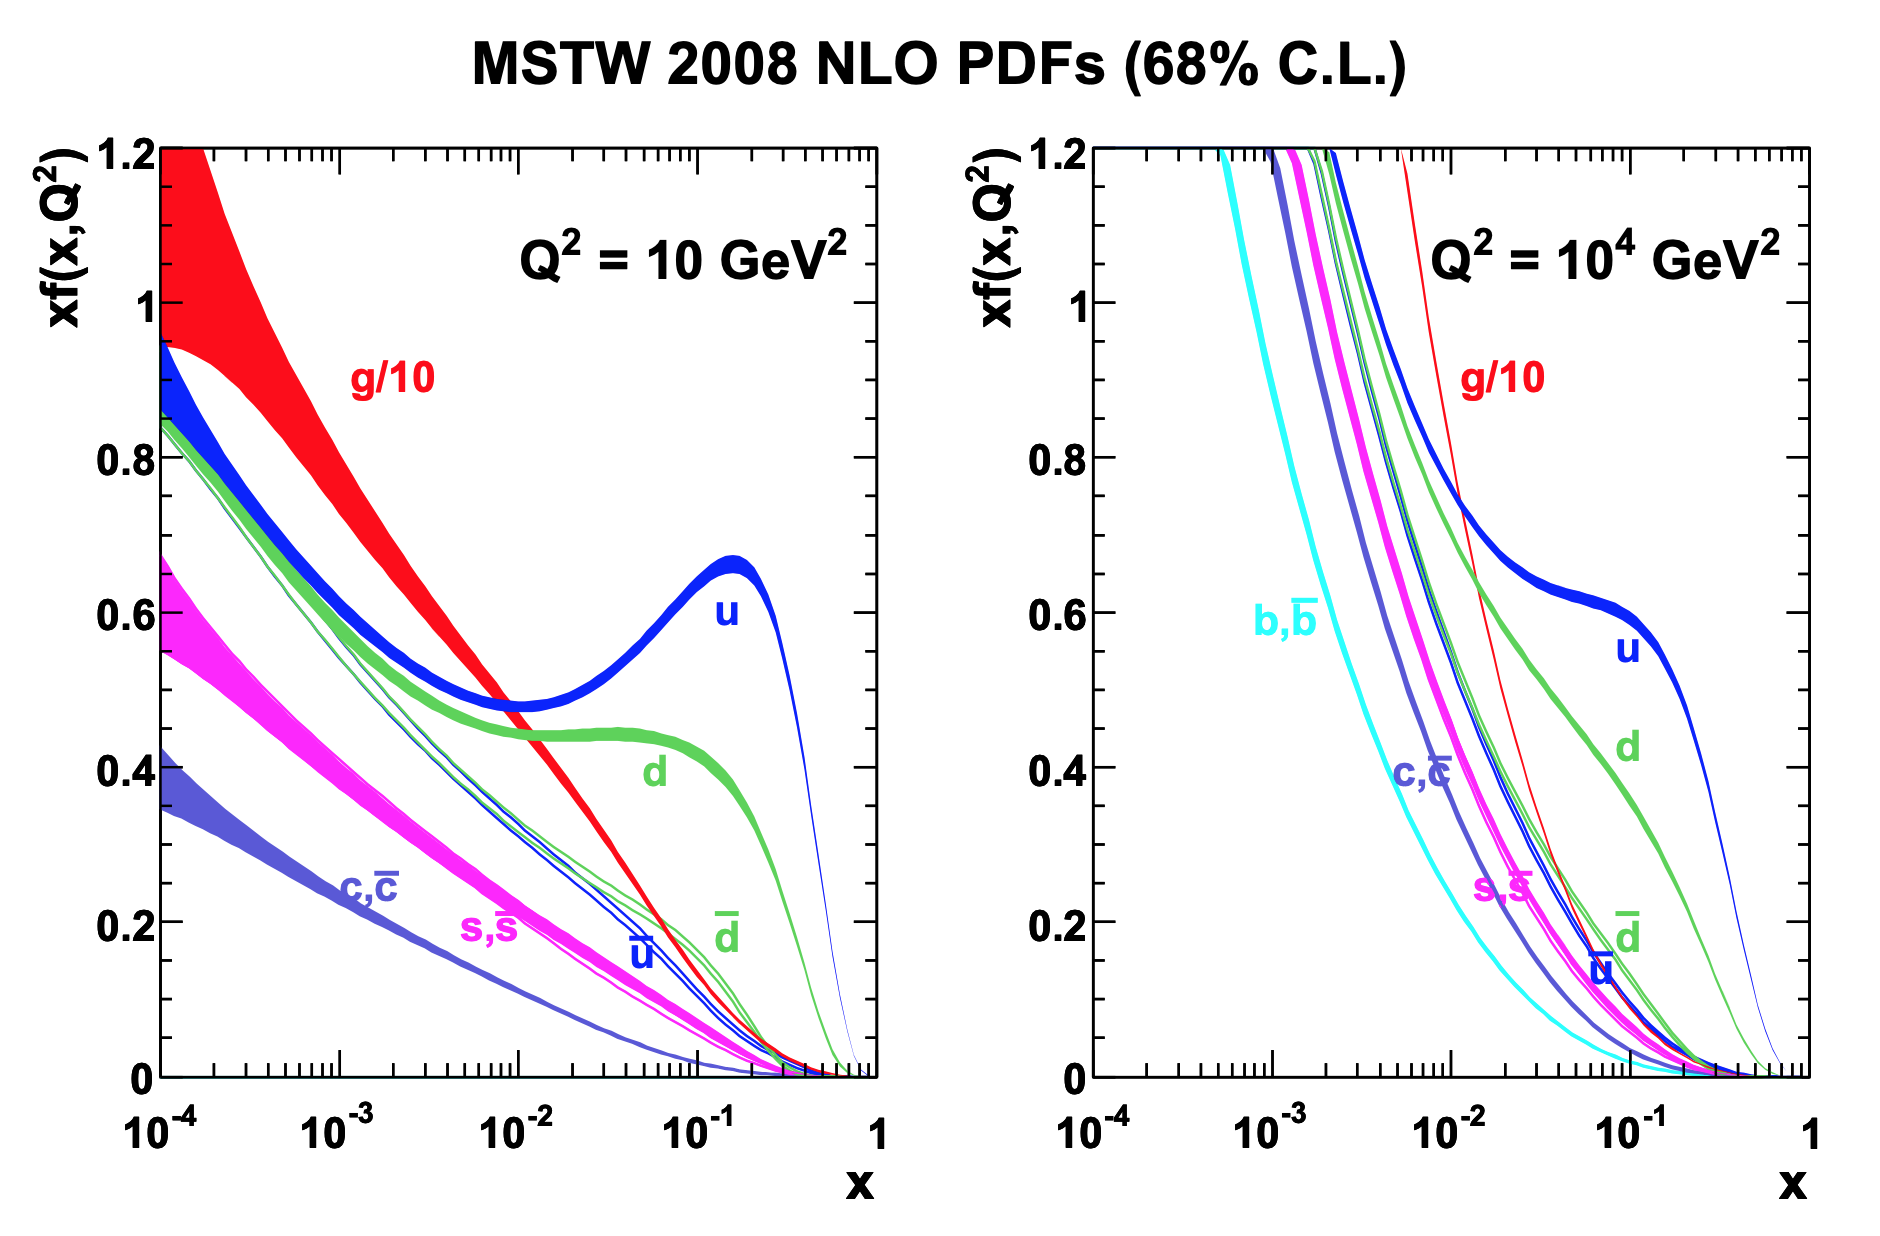
\includegraphics[width=\linewidth]{figures/physics_of_pp/pp_nlo_pdfs.png}
    \caption{Parton distribution functions for the proton, shown for $Q^2 = 10$ GeV (left) and $Q^2 = 10^4$ GeV (right), as calculated by the MSTW group. The width of each band indicates the 68\% C.L. Taken from~\cite{Martin:2009iq}.}
    \label{fig:pp_nlo_pdfs}
\end{figure}
Although the proton's quantum numbers are determined by its valence quarks, $uud$, there is a non-negligble fraction of the proton's momentum carried by both the gluons and the ``sea'' of quark-antiquark pairs.
